\documentclass[10pt]{article}

\title{Running biomechanics and the effect of heel versus forefoot strike}
\author{John Trombetta\thanks{Author is with the Department of Mechanical Engineering at the United States Naval Academy. Address for correspondence: \emph{m236348@usna.edu}}}
\date{\today}


\usepackage[separate-uncertainty=true]{siunitx}
\DeclareSIUnit{\year}{y}
\DeclareSIUnit{\inch}{in}
\DeclareSIUnit{\foot}{ft}
\DeclareSIUnit{\poundforce}{lbf}
\DeclareSIUnit{\pound}{lb}
\DeclareSIUnit{\frame}{frame}
\usepackage{graphicx}
\usepackage[round,authoryear]{natbib}
\bibliographystyle{apalike}
\usepackage[plain]{fancyref}
\usepackage{listings}
\usepackage{amsmath,amsfonts,amssymb}
\usepackage{booktabs}
\lstset{%
  basicstyle=\ttfamily,
  columns=fullflexible,
  showstringspaces=false}
\usepackage[dvipsnames,svgnames]{xcolor}
\usepackage{hyperref}
\hypersetup{%
  colorlinks=true,
  linkcolor=violet,
  urlcolor=blue,
  citecolor=blue}
\usepackage{svg}
%\usepackage{svg-extract}
\usepackage{fullpage}
\newcommand{\Homosapiens}{\emph{Homo sapiens}}
\newcommand{\Hsapiens}{\emph{H.~sapiens}}
\newcommand{\Matlab}{Matlab}




\begin{document}
\maketitle
\begin{abstract}
Write one paragraph here that explains what your report is about.
\end{abstract}
{\scriptsize\textbf{Keywords: }shin splints, running, kinematics, ground reaction forces, kymograph}

\section{Introduction}
% Trombetta: Most of what I have is not running shin splints stuff; hopeful you found some there. I do have some general human running stuff in the list. You might ask 1/C Anmol Walha about running biomechanics, and 1/C Lily Bautista about walking and ankles? I have their 485 projects but not the references they found... 
%Work from an inverted triangle (broader topics to more specific). Explain what you are interested, review some relevant literature, and then set up what your specific research question is. Cite literature using the author-year format, as in \citep{buck2020go}. If you need pictures to explain the relevant biomechanics, feel free to include. This section should also say a little why your research matters. The last part of this section should be the specific hypotheses you seek to test. 

%What is shin splint? 
%To study the effectiveness and injury risk of heel strike versus forefoot strike running.
\citet{slocum1967shin} medically described shin splints as a symptom complex characterized by pain and discomfort in the lower leg after repetitive overuse in walking or running. The usual sites of pain are the lower half of the posteromedial border of the tibia, the anterior tibial compartment, the tibia, and the interosseous membrane; other additional technical details are provided to distinguish it from stress fractures, anterior tibial syndrome, and muscle hernia \citep{slocum1967shin}. As a midshipman in my first year at the United States Naval Academy, I am acutely familiar with repetitive overuse of the lower leg in waking and running, which motivates me to understand how biomechanics may play a role in avoiding shin splints. 

\subsection{Potential for running style to reduce risk of shin splints}
%Explain heel strike versus forefoot strike
One potential avenue to reduce shin splints is running style. Heel-strike is a style in which the initial contact of the foot with the ground, at the beginning of the stance phase, is made using the heel. In contrast, forefoot-strike involves using the ball of the foot or other midfoot parts. Popular press articles for runners discuss the potential for running style in reduce or prevent injuries \citep{douglas2012midfoot, giandolini2013impact}, while the general biomechanics of running is reviewed in \citep{chan1994foot, lieberman2020biomechanical, bramble2004endurance, lieberman2010foot}. 

What is the evidence that suggests forefoot-strike and similar styles might help with shin splints? \citet{larson2014comparison} examined barefoot and minimally shod runners in a recreational road race and found only 20.7\% of barefoot runners were rearfoot (heel) strikers. \citet{gans1985relationship} studied ballet dancers and found that dancers with a history of shin splints demonstrated more double heel strikes when executing a sequence of jumps. In an Army study, \citet{diebal2012forefoot} found a 6-week forefoot strike running intervention reduced pain and disability associated with chronic exertional compartment syndrome. \citet{willems2004intrinsic} conducted a study with 400 physical education students and found subjects that developed exercise-related lower leg pain had an altered running pattern compared to the controls including a more central heel strike. 

On the other hand, \citet{cibulka1994shin} presented a case study of a patient with shin splints who ran using a forefoot contact running style, whose symptoms were resolved when shifting to a heel-toe style. In another Army study, \citet{warr2015characterization} characterized foot-strike patterns in 341 soldiers and found no difference between injury rates or performance on a two-mile run between heel-strike and nonheel-strike. \citet{thacker2002prevention} states that use of shock-absorbent insoles, foam heel pads, heel cord stretching, alternative footwear, as well as graduated running programs among military recruits have undergone assessment in controlled trials, which have not shown strong support for any of these interventions. \citet{thacker2002prevention} concluded that the literature yielded little objective evidence to support widespread use of any existing interventions to prevent shin splints, and suggested a rigorously implemented research program is critically needed to address this common sports medicine problem.




\subsection{Are there observable biomechanical differences between running styles that may reduce the risk of shin splints?}

My guiding research question is, what relevant and quantitaive biomechanics observations can I make regarding between running styles?  While the global COVID-19 pandemic limited my access to lab instrumentation, studies of human running gait and biomechanics historically made use of clever improvised methods to provide insight \citep{baker2007history, mcmahon1984muscles, mayer2010physiological, marey1873locomotion, carlet1872essai, muybridge1901human}. In particular, early studies made clever use of photography \citep{muybridge1901human, baker2007history, mcmahon1984muscles, mayer2010physiological} and wearable instrumentation \citep{marey1873locomotion, carlet1872essai, baker2007history, mayer2010physiological}. The wearable instrumentation available to early researchers (\fref{fig:intro}) included the kymograph, in which movement of limbs or pressure of the feet were use to actuate a stylus and inscribe records of force or motion, for example, on a soot blackened glass slide or cylinder. More modern versions of this instrumentation have been used as a cheap way to record maximal flows and forces using instrumentation deployed in the intertidal zone in heavy California surf \citep{bell1984quantifying, denny1983simple}.
\begin{figure}
\begin{center}
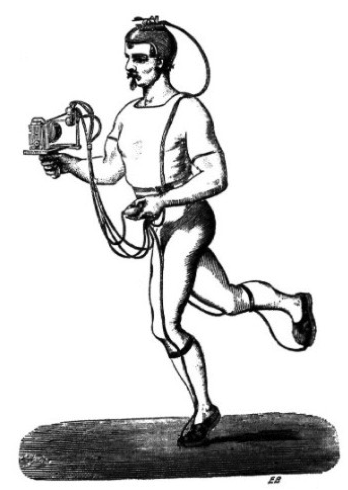
\includegraphics[height=1.5in]{figures/intro3.png}\hspace{0.5in}
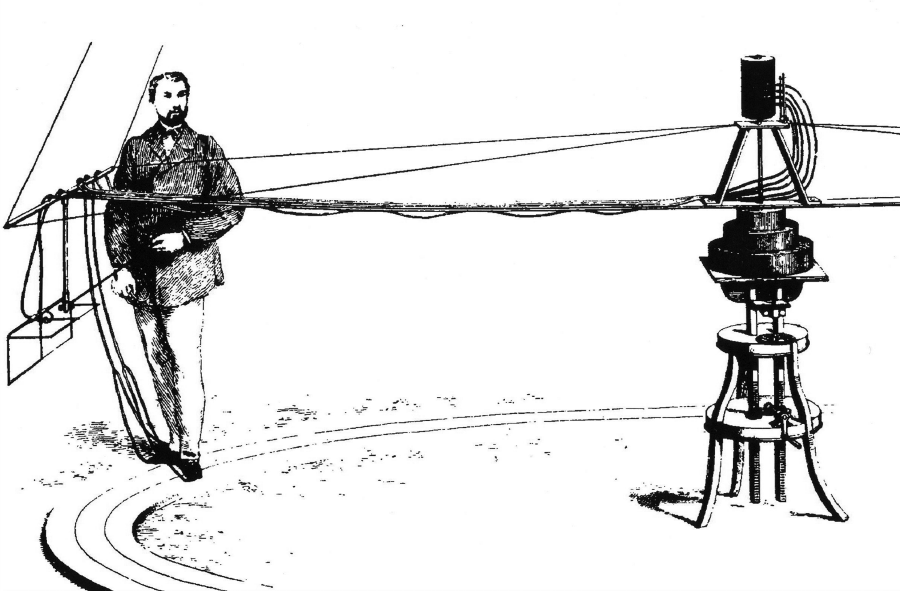
\includegraphics[height=1.5in]{figures/intro4.png}
\end{center}
\caption{Early wearable instrumentation applied to running biomechanics, from \citep{marey1873locomotion, carlet1872essai}. Tubes, mechanical linkages, and other contrivances were used to actuate a stylus, providing a record of stride frequency, angles, forces, or other data.} 
\label{fig:intro}
\end{figure}

I hypothesize that the apparent reduced risk of shin splints in forefoot strike / toe-strike could be due to lower overall forces or accelerations, as measured using a force plate or wearable accelerometer. Alternatively, the overall forces and accelerations may be similar between the two styles, but may have fine kinematic details that suggest a mechanism for clinical observations regarding running style. 



 %\section{Introduction}
\section{Methods and materials}
\label{sec:methods}

Data and source code for analyses and plots are available in a Github repository at: \url{https://github.com/ew282d-evangelista/ew282d-sp2020-0451-trombetta}.

\subsection{Experimental subject}
I used a single experimental subject, age \SI{19}{\year}, male, height \SI{5}{\foot} \SI{10}{\inch} (\SI{1.78}{\meter}), mass \SI{150}{\pound} (\SI{68.0}{\kilo\gram}). For this subject, measured hip height from the ground was \SI{36}{\inch} (\SI{0.91}{\meter}). For scale purposes, the subject shoe size was US9.5M, heel to toe length \SI{0.30}{\meter}. During running trials, the subject wore physical training gear consisting of running shorts, a tshirt, white ankle socks, and athletic shoes (Lunarlite; Nike, Beaverton, OR) \textbf{FIX} with high contrast black uppers and a white sole and heel that aided in manual digitization. The subject was in good physical condition, having completed his first year as a midshipman at the US Naval Academy, including its renowned Physical Education Program. The subject provided his informed consent before measurements\footnote{This pilot study was conducted under the following exemption: The project in EW282D is designed to teach research methods through student interaction with data about individuals. Student class assignments typically do not meet the federal regulatory definition of research, thus do not require institutional review board application, approval, or oversight.}.  

\textbf{How was subject trained to do heel strike versus toe strike (foot strike) running styles?}



\subsection{Improvised force plate kymograph}
To measure horizontal and vertical ground reaction forces (GRFs), I originally intended to use a three-axis force plate (9260AA6; Kistler; Novi, MI), however, due to the global COVID-19 pandemic, the equipment was not available. Instead, I improvised a one-axis (vertical only) force plate (\fref{fig:methods:forceplate}) using a flexure made of a \SI{48 x 21 x 0.5}{\inch} sheet of scrap bead board simply supported at the ends between two masonry pavers each \SI{2.25}{\inch} thick. I attached a red dry erase marker (EXPO; Newell Brands; Atlanta, GA) horizontally, pointing laterally, at the midpoint of the flexure, so that the marker would mark a \SI{11x14}{\inch} whiteboard (Staples; Riverdale, NJ) on the right side. 
\begin{figure}
\begin{center}
    \textbf{Fill in.}
\end{center}
\caption{Improvised one-axis force plate kymograph}
\label{fig:methods:forceplate}
\end{figure}
The lowest point reached by the marker is a linear measure of the maximum vertical GRF experienced during contact. Additionally, I found that horizontal GRF would displace the flexure horizontally, providing some indication of their general magnitude. \textbf{Add refs to Malet etc, Denny.} For a point load applied in the middle, the displacement $\delta$ (i.e. marker movement) from point load $F$ (i.e. vertical GRF) is given by: % ADD CITATION
\begin{equation}
\delta = \frac{FL^3}{48 EI},
\label{eq:sensor-response}
\end{equation}
where $E$ is Young's modulus of elasticity, $L$ is the length of the beam, and $I=\frac{1}{12}bh^3$ is the second moment of area; though in practice I simply compared the maximum marker motion rather than perform a detailed calibration of this improvised rig. 

\textbf{How many steps and in what order.} After each trial, the resulting marker pattern on the white board was photographed using a smartphone camera (Iphone 11; Apple; Cupertino, CA) to allow rough comparison of the magnitude of vertical GRF. 



\subsection{Measurement of accelerations using a smart phone}
In addition to the rough indication of vertical GRF from the improvised force plate, I measured accelerations in three axes using a smartphone (iPhone 5s; Apple; Cupertino, CA), centered \SI{10}{\centi\meter} below the navel and held in place with the right hand. I used the \Matlab\ Mobile app (Mathworks; Natick, MA) to log $X$, $Y$, and $Z$ acceleration at a sampling rate of \SI{100}{\hertz}.  Running was conducted moving straight and level on an empty street about two blocks in length. I recorded \SI{45}{\second} samples of steady running using each running style, at a cadence of approximately \SI{150}{steps\per\minute}, timed using the Avril Lavigne song ``Sk8er Boi''. To avoid end effects during start and stop, I used the middle \SI{10}{\second} segment of each recording for analyses of the acceleration of the center of mass. Analysis of the vertical ($Y$) acceleration measurements was carried out \Matlab (Mathworks; Natick, MA) and R \cite{r2020}, including the \lstinline{tidyverse} and \lstinline{ggplot2} libraries \citep{wickham2019tidyverse}. 



\subsection{Video kinematics on a treadmill}
To examine changes in kinematics and gait during the different running styles, I filmed the subject running on a treadmill (Performance 800; TRUE Fitness; St Louis, MO). Ideally I would have used a high speed camera (TS5; Fastec; San Diego, CA), however, COVID-19 required me to improvise. Instead, I used a smartphone camera (iPhone 11; Apple; Cupertino, CA) filming from the left at \SI{1}{\meter} \textbf{FIX}. The camera operated at \SI{30}{\frame\per\second} and \num{1920x1080} pixel resolution. The treadmill was operated at \SI{8}{mph} (\SI{3.6}{\meter\per\second}) for both tests; the subject began running on the treadmill and reached a steady pace before filming.  Two segments were obtained for analysis, \SI{11}{\second} and \SI{13}{\second} in length, for heel-strike and toe-strike styles, providing \SI{358}{\frame} and \SI{416}{\frame}, respectively.
\begin{figure}
\begin{center}
    \textbf{Fill in.}
\end{center}
\caption{Need a figure of example setup, points digitized, and maybe angles annotated.}
\label{fig:methods:kinematics}
\end{figure}

Kinematic analysis proceeded using \citet{hedrick2008software} DLTdv8 (\url{http://biomech.web.unc.edu/dltdv/}) to manually digitize six points (\fref{fig:methods:kinematics}) in each frame of video: (1) left toe at the front of the white sole; (2) left heel at the back of the white sole; (3) left ankle at the lateral malleolus as judged by white ankle socks worn by the subject; (4) left knee as judged by the bump from the lateral condyles of the femur and tibia; (5) left hip as judged from a faint stripe marking on the subject's athletic shorts. In addition, a sixth point, the right toe, was also digitized in order to confirm that the left-right phase was \ang{90}. 

Specially written code in \Matlab\ was used to convert the digitized point locations into the joint angles depicted in \fref{fig:methods:kinematics}. Foot angle ($\alpha$) was defined with \ang{0} as anatomically neutral position, positive $\alpha$ as dorsiflexion, and negative $\alpha$ as plantar flexion. The knee angle ($\beta$) was defined with \ang{0} as anatomically neutral position, and positive $\beta$ as knee flexion. Hip angle ($\gamma$) was defined with \ang{0} as anatomically neutral position, positive $\gamma$ as flexion, and negative $\gamma$ as extension. 

In addition to joint angle, phase was recovered using a method based on the Phaser algorithm \citep{revzen2008estimating}, by taking the principal component analysis (PCA) of all the six digitized points' $x$ and $y$ coordinates, then finding the phase angle of the Hilbert transform of the first principal component (PC1). The phase was then adjusted to range from 0 to $2\pi$, with 0 phase corresponding to the beginning of the first recorded stance phase. This allows comparison of each of the \textbf{FILLIN} and \textbf{FILLIN} steps in the heel-strike and toe-strike analysis videos, respectively. Phase calculations were carried out in \Matlab\ and made use of the \lstinline{pca} and \lstinline{hilbert} functions. 

To allow for comparison of stride frequency, stride period, and duty cycle, the videos were reviewed frame by frame in DLTdv8 to identify (1) the start of stance phase based on toe or heel contact; (2) end of stance phase judged by toe liftoff; and (3) toe contact (for heel-strike trials) to aid in length and speed calibration.  For heel-strike analysis, start of stance was judged by heel-strike and rapid foot plantar flexion in contact with the ground; for toe-strike analysis, start of stance was judged by observing when the toe struck the ground during plantar flexion. The angle from the point of contact (heel or toe) to the hip, and the angle of the ankle were also computed as part of this analysis. Additional plotting and statistical analyses were completed in \Matlab\ and R \citep{r2020}. 


 %\section{Methods and materials}
\section{Results}
\label{sec:results}
%Explain factually what you found... leave interpretation of what it means for the final discussion section. Here you would include plots of what you found or comparison tables.

\subsection{Improvised force plate kymograph}
Heel versus toe-strike two trials. Toe-strike only shows lateral movement of rig, primarily with left foot. 
\begin{figure}
\begin{center}
\textbf{Fill in from slides 11 and 12.}
\end{center}
\caption{Improvised force plate recordings of vertical ground reaction force; (a) and (b) trials comparing heel strike and toe strike; (c) checking toe strike.}
\label{fig:results:forceplate}
\end{figure}

\subsection{Measurements of acceleration using a smartphone}

\subsection{Video kinematics on a treadmill}
 %\section{Results}
\section{Discussion}
\label{sec:discussion}

\subsection{Heel- and toe-strike do not appear to produce different vertical ground reaction forces (GRF) or body accelerations}

One hypothesis I set out to test was that heel-strike would produce larger ground reaction forces (GRFs) or body accelerations. This was not supported by data from the force plate kymograph (\fref{fig:results:forceplate}) or from body center of mass accelerations during running (\fref{fig:results:accel}, which showed little difference between the vertical GRFs and $Y$ component accelerations. As a result, I conclude shin splints are not just caused by grossly higher forces in heel-strike running. In retrospect, it seems reasonable to expect this as the weight of the runner has not changed and the overall stride parameters (stride frequency, period, length, and duty cycle), while posessing some small changes, are not wildly different (\fref{fig:results:stride} and \fref{tab:results:stride}). 



\subsection{Toe-strike (forefoot strike) may produce larger horizontal GRFs on pushoff?}

The force plate kymograph data suggest that toe- forefoot strike produces a larger horizontal ground reaction force upon pushoff. The improvised instrumentation I used was too crude to observe the magnitude and timing of horizontal ground reaction forces; and an alternative explanation could be that the pavers used in the force plate have nonlinear friction in one direction that resulted in the observed patterns (yellow arrows in \fref{fig:results:forceplate}). However, given that for the same speed, toe-striking used a shorter duty cycle (\fref{fig:results:stride} and \fref{tab:results:stride}) it seems reasonable that, with less contact time with the ground per step, the horizontal ground reaction forces to keep moving forward at the same speed would need to be higher during some part of the cycle.



\subsection{Kinematic differences between heel- and toe-strike suggest a mechanism for higher loads in the lower leg}

Without a ``smoking gun'' in my force plate and accelerometer readings, I had to take a closer look at kinematic differences between the two running styles. The hip and knee joint angles look similar between the heel- and toe-strike (\fref{fig:results:jointangles}C-F), however, there are clear differences in the foot angles (\fref{fig:results:jointangles}A-B). In heel-strike, the leg impacts the ground with the heel, while the foot is dorsiflexed. During toe-strike, on the other hand, the leg impacts the ground with the toe, and the foot remains plantar flexed for nearly all of stance.

When I look closely at the kinematic tracings of figures~\ref{fig:results:heelpretty} and \ref{fig:results:toepretty}, it appears that during heel-strike as the heel comes in contact with the ground, the lower leg (knee to ankle, containing tibia, fibula, etc) is closely aligned with the line of action of the ground reaction force to the hip (compare line from hip to triangles versus the alignment of the lower leg in \fref{fig:results:heelpretty}). In contrast, during toe-strike as the toe comes in contact with the ground, the lower leg is not aligned with the line of action of the ground reaction force to the hip (line from hip to triangle is not aligned with lower leg in \fref{fig:results:toepretty}). When I compared these angles (\fref{fig:results:contactangles}), the differences between the two treatments were significant. While the gross, overall forces and accelerations may not be different between the two styles, the fine details of forces as experienced by particular parts of the leg could be very different during key instances of the stride; in heel-strike the lower leg must take all of the load as a compressive shock load at the start of every stance phase, while in toe-strike the leg acts more compliant and is able to share the load not just on the lower leg, but also the foot, the upper leg, and the muscles and tendons crossing several joints. 

\textbf{Wrap up here. Cite others and put your work in context...} The data in other studies show that heel strikes produce a larger more instantaneous impact causing injuries compared to a slower more spread out force with a forefoot strike. 

\citet{dickinson1985measurement} demonstrated a shock wave propagates through the skeletal system following heel strike and suggests it was not seen in previous measurements because of adequate shock absorption provided by running shoes, but became readily apparent in barefoot runners. 

\citet{knorz2017three} combined left and right force plate measurements and 3D kinematics to resolve the detailed ground reaction forces and to map them to stress patterns in the ankle, knee, and hip joint, concluding that forefoot and rearfoot strike were associated with different 3D stress patterns with no global advantage of one strike pattern over the other. Rearfoot strike had peak during initial contact as seen in the (HARVARD DATA) but had a lower maximum peak force during stance.

\citet{viitasalo1983some} found runners with shin splints had greater angular displacements and experienced greater Achilles tendon angles during shin splints, as well as greater angular displacement between heel strike and the maximal everted position. 

\citet{giandolini2013impact} found a combination of compliant shoes, increased stride frequency, and shifting to a forefoot strike were effective in attenuating the foot-ground impact. They also found that forefoot strike was associated with pre-activation of the gastrocnemius lateralis, preparing it to act as a spring or shock absorber during contact. 

\citet{mizrahi2000effect} found that kinematic changes in long distance runners during fatigue included lower stride frequency, joint angle differences, increased hip vertical excursion, and higher accelerations of the shank, which they interpreted as conssitent with higher impact accelerations and increasd risk of overload injuries. 

The joint angles I observed were similar to those in high speed walking \citep{liu2008muscle}. 

Impact peak seen in \citep{chan1994foot, boyer2015rearfoot}.

\citet{boyer2015rearfoot} concluded that not all lower extremity loading variables are lower with a forefoot strike or when running barefoot; switching to a forefoot strike may not alleviate certain pain or help runners avoid injury. A more viable option may be to shorten one’s stride length 10\% \citep{boyer2015rearfoot}.

Adoption of a more compliant gait might be expected to reduce mechanical forces transmitted through the skeleton but incurs a higher metabolic cost \citep{mcmahon1987groucho}. 



 %\section{Discussion}

\section{Acknowledgements}
I thank Cameron Smith, Alexis Pak, and Sofia Figueroa for their assistance as classmates in EW282D / EW496. USNA Biomechanics is supported by Lockheed Martin. 

% References
\bibliography{trombetta.bib}

%\clearpage
%\appendix
%\renewcommand{\figurename}{Supplementary Figure}
%\renewcommand{\thefigure}{S\arabic{figure}}
%\input{method-details.tex}
\end{document}
